%====================== header ==================================================
\documentclass[12pt]{osuthesis}

%====================== process the document configuration ======================
%====================== font dependent settings
\renewcommand{\labelitemi}{$\bullet$}

%====================== provides some shapes, not necessarily used directly =====
\usepackage{pict2e}

%====================== get rid of tiny overfull box warnings ===================
\hfuzz=3pt

%====================== create an execute function so we can shell out ==========
\def\execute{%
    \begingroup
    \catcode`\%=12
    \catcode`\\=12
    \executeaux}
\def\executeaux#1{\immediate\write18{#1}\endgroup}

%====================== indexing ================================================
\usepackage{makeidx} %index package
\execute{makeindex main}
\makeindex

%====================== nomenclature ============================================
\usepackage{nomencl}
% nomenclature subgroup syntax
% B = subscript
% P = superscript
% R = roman symbols
% G = greek symbols
%originally we had the nomgroup redefinition here, but it needs to be in the same
%  document as the printnomenclature command...or so it seems
%convert the .nlo list into the proper nomenclature
% environment in .nls by using style nomencl.ist
\execute{makeindex main.nlo -s nomencl.ist -o main.nls}
\makenomenclature

%====================== bibliography ============================================
\usepackage[round]{natbib} %bibliography citation style with round brackets

%====================== AMS math packages =======================================
\usepackage{amsmath}
\usepackage{amsxtra}
\usepackage{amstext}
\usepackage{amssymb}

%====================== Tables, figures =========================================
\usepackage{array}
\usepackage{subfig}
\usepackage{rotating}

%====================== Units package ===========================================
\usepackage[squaren]{SIunits}

%====================== Other packages ==========================================
\usepackage{graphicx} %convenient graphics import package
\usepackage{ifthen}       %Add ifthenelse support
\usepackage{enumerate} %modify enumerate style
\usepackage[usenames,dvipsnames]{xcolor}
\usepackage[colorlinks,citecolor=Black,linkcolor=Black,urlcolor=Black,filecolor=Black]{hyperref}
\usepackage{url} % allow typsetting urls
\usepackage{setspace} % allow easy variation of line spacing
\usepackage{lipsum}

%====================== margin comments ========================================
\setlength{\marginparwidth}{1.0in}
\setlength{\marginparsep}{0.1in}
\let\oldmarginpar\marginpar
\renewcommand\marginpar[1]{\-\oldmarginpar[\raggedleft\tiny #1]{\raggedright\scriptsize\color{red} #1}}

%============ tell LaTeX where to find images ===================================
\graphicspath{
              {Ch-Introduction/images/}
              {Ch-Methods/images/}
              {Ch-Results/images/}
             }

%============ specify how deep layout numbering goes ============================
\setcounter{secnumdepth}{3} %3 specifies to number down to subsection
\setcounter{tocdepth}{3} %3 specifies to include down to subsections in the TOC

%============ hack to add leader dots to the TOC chapters ========================
\usepackage{etoolbox}
 \makeatletter
 \patchcmd{\l@chapter}
   {\hfil}
   {\leaders\hbox{\normalfont$\m@th\mkern \@dotsep mu\hbox{.}\mkern \@dotsep mu$}\hfill}
   {}{}
 \makeatother


%====================== read any new commands or environments ===================
%% User defined commands here

\newcommand{\RB}[1]{\left[#1\right]}
\newcommand{\PB}[1]{\left(#1\right)}
\newcommand{\SB}[1]{\left|#1\right|}
\newcommand{\CB}[1]{\left\{#1\right\}}

%\let\origitemize\itemize
%\renewenvironment{itemize}{\origitemize\setlength{\itemsep}{1pt}\setlength{\parskip}{0pt}\setlength{\parsep}{0pt}}{\endlist}
%
%\let\origdescription\description
%\renewenvironment{description}{\origdescription\setlength{\itemsep}{1pt}\setlength{\parskip}{0pt}\setlength{\parsep}{0pt}}{\endlist}
%
%\let\origenumerate\enumerate
%\renewenvironment{enumerate}{\origenumerate\setlength{\itemsep}{1pt}\setlength{\parskip}{0pt}\setlength{\parsep}{0pt}}{\endlist}
%
%\newenvironment{chapterAbstract}
%    { %before environment contents...
%      \begin{quote}
%        \begin{flushleft}
%            \begin{Large} Abstract \end{Large}
%        \end{flushleft}
%        \vspace{-1em}
%        \hrulefill
%        \vspace{-1.7em}
%        \begin{singlespacing}
%    }
%    { %after environment contents...
%         \end{singlespacing}
%        \vspace{-1em}
%        %\hrulefill
%      \end{quote}
%    }
%
\newenvironment{dedication}
   {\vspace{6ex}\begin{quotation}\begin{center}\begin{em}}
   {\par\end{em}\end{center}\end{quotation}}

%====================== document information ====================================
\title{THIS IS THE NAME OF MY THESIS}

\formattedtitle{THIS IS THE \\ NAME OF MY THESIS}

\author{JOHN Q. DOE}

\degreeone{\ssp B.A. \\
        Oklahoma State University\\
        Stillwater, OK, USA\\
        2014}

\degreetwo{\ssp M.S. \\
        Oklahoma State University\\
        Stillwater, OK, USA\\
        2017}

\degreesought{Doctor of Philosophy}

\degreedate{May 2018}

\majorfield{Rocket Science}


\begin{document}

%====================== make title page =========================================
\maketitle

%====================== make approval page ======================================
\makeapproval{4} % use this for the page your committee will sign
%\makeElectronicapproval{4} % use this page for the electronic thesis submission

%====================== make acknowledgments page ===============================
\begin{acknowledge}
	\begin{acknowledge}
To all the little people...	

    \clearpage
    \vspace{3in}
    \begin{dedication}
    Get your facts first, then you can distort them as you please. \\ ---Mark Twain
    \end{dedication}

\end{acknowledge}

\end{acknowledge}

%====================== make dedications page ===============================
\begin{dedication}
    \vspace*{\fill}
Get your facts first, then you can distort them as you please. \\ ---Mark Twain
\vspace*{\fill} 

\end{dedication}

%====================== make abstract ===========================================
\renewcommand{\thepage}{\roman{page}}
\begin{abstract}{JOHN Q. DOE}{ROCKET SCIENCE}
    This study reports how to herd sheep on Mars. The results are intriguing and very important to future interplanetary biology.

\end{abstract}

%====================== table of contents creation ==============================
%\addtocontents{toc}{\conttocheading}  %% uncomment this line for multipage TOC
\tableofcontents

%====================== table of tables creation ================================
%\addtocontents{lot}{\conttotheading}  %% uncomment this line for multipage LOT
\listoftables

%====================== list of figures creation ================================
%\addtocontents{lof}{\conttofheading}  %% uncomment this line for multipage LOF
\listoffigures

%====================== abbreviations============================================
\begin{abbreviation}
	\begin{longtable}{p{.20\textwidth} p{.70\textwidth}}
AC & Alternating Current \\
GM & General Motors \\
OK & Oklahoma \\
\end{longtable}

\end{abbreviation}

%====================== nomenclature ============================================
\begin{nomenclature}
	
%====================== nomenclature -- must be customized here ===================
% ==== Redefine the command called for sorting the nomenclature
\renewcommand{\nomgroup}[1]
    {%
     \ifthenelse{\equal{#1}{R}}{\vspace{0.3cm}\item[\textbf{Variables}]}{
      \ifthenelse{\equal{#1}{G}}{\vspace{0.3cm}\item[\textbf{Greek Symbols}]}{
       \ifthenelse{\equal{#1}{B}}{\vspace{0.3cm}\item[\textbf{Subscripts/Superscripts}]}{
       }
      }
     }
    }
% ==== Redefine the length between items in the nomenclature
\setlength{\nomitemsep}{-\parsep}
% ==== Redefine the page to be roman numerals
\renewcommand{\thepage}{\roman{page}}
% ==== Set the value of page to the value of placeholder...which is apparently
%      passed from the previous environment
\setcounter{page}{\value{placeholder}}
% ==== Redefine the nomenclature name to be more inline with other dissertation environments
\renewcommand{\nomname}{\centering \ssp \rule{0in}{1in} \par
    NOMENCLATURE \par
    \vspace*{0.25in} \par \dsp}
% ==== Add a preamble statement to the nomenclature
%\renewcommand{\nompreamble}{The following is a list of symbols, variables, and scripts used in this work which may not be defined as they are encountered in the body.}
% ==== Redefine the nomenclature label to have trailing dots filling up the box
\renewcommand{\nomlabel}[1]{#1\nobreakspace\dotfill}
% ==== Print the nomenclature to the pdf
{\ssp \printnomenclature[0.75in]}

\nomenclature[aA ]{$A$}{Surface area}
\nomenclature[ac ]{$C_p$}{Specific heat}
\nomenclature[ae ]{$e'$}{Vapor pressure deficit of the air}
\nomenclature[aE ]{$E$}{Rate of evapotranspiration from the surface}
\nomenclature[aGr]{$G_r$}{Net radiation into the surface}
\nomenclature[aN ]{$N$}{Number or count of a material or property}

\nomenclature[g1 ]{$\alpha$}{Thermal diffusivity}
\nomenclature[g3 ]{$\gamma$}{Psychrometric constant}

\nomenclature[b0 ]{$0$}{Initial condition}
\nomenclature[ba ]{$a$}{Property of the air}
\nomenclature[bc ]{$c$}{Radial centroid}


\end{nomenclature}

%====================== main  body of the dissertation ==========================
% ==== Get a new page to leave the last page of the nomenclature unaffected
\newpage
% ==== Set line spacing for the bulk of the document
%\setstretch{1.4}
\doublespacing
% ==== Reset page numbering to arabic numerals...this also resets it to start at 1
\pagenumbering{arabic}


%====================== chapters information ====================================
\chapter{Introduction}
\label{ch:Introduction}

Due to the interesting work done by \cite{ABDELFETTAH20181}, and \cite{SCARLAT20151269}, we are able to...

\section{Reason for Study}

\lipsum[1]

\begin{figure}
    \centering
    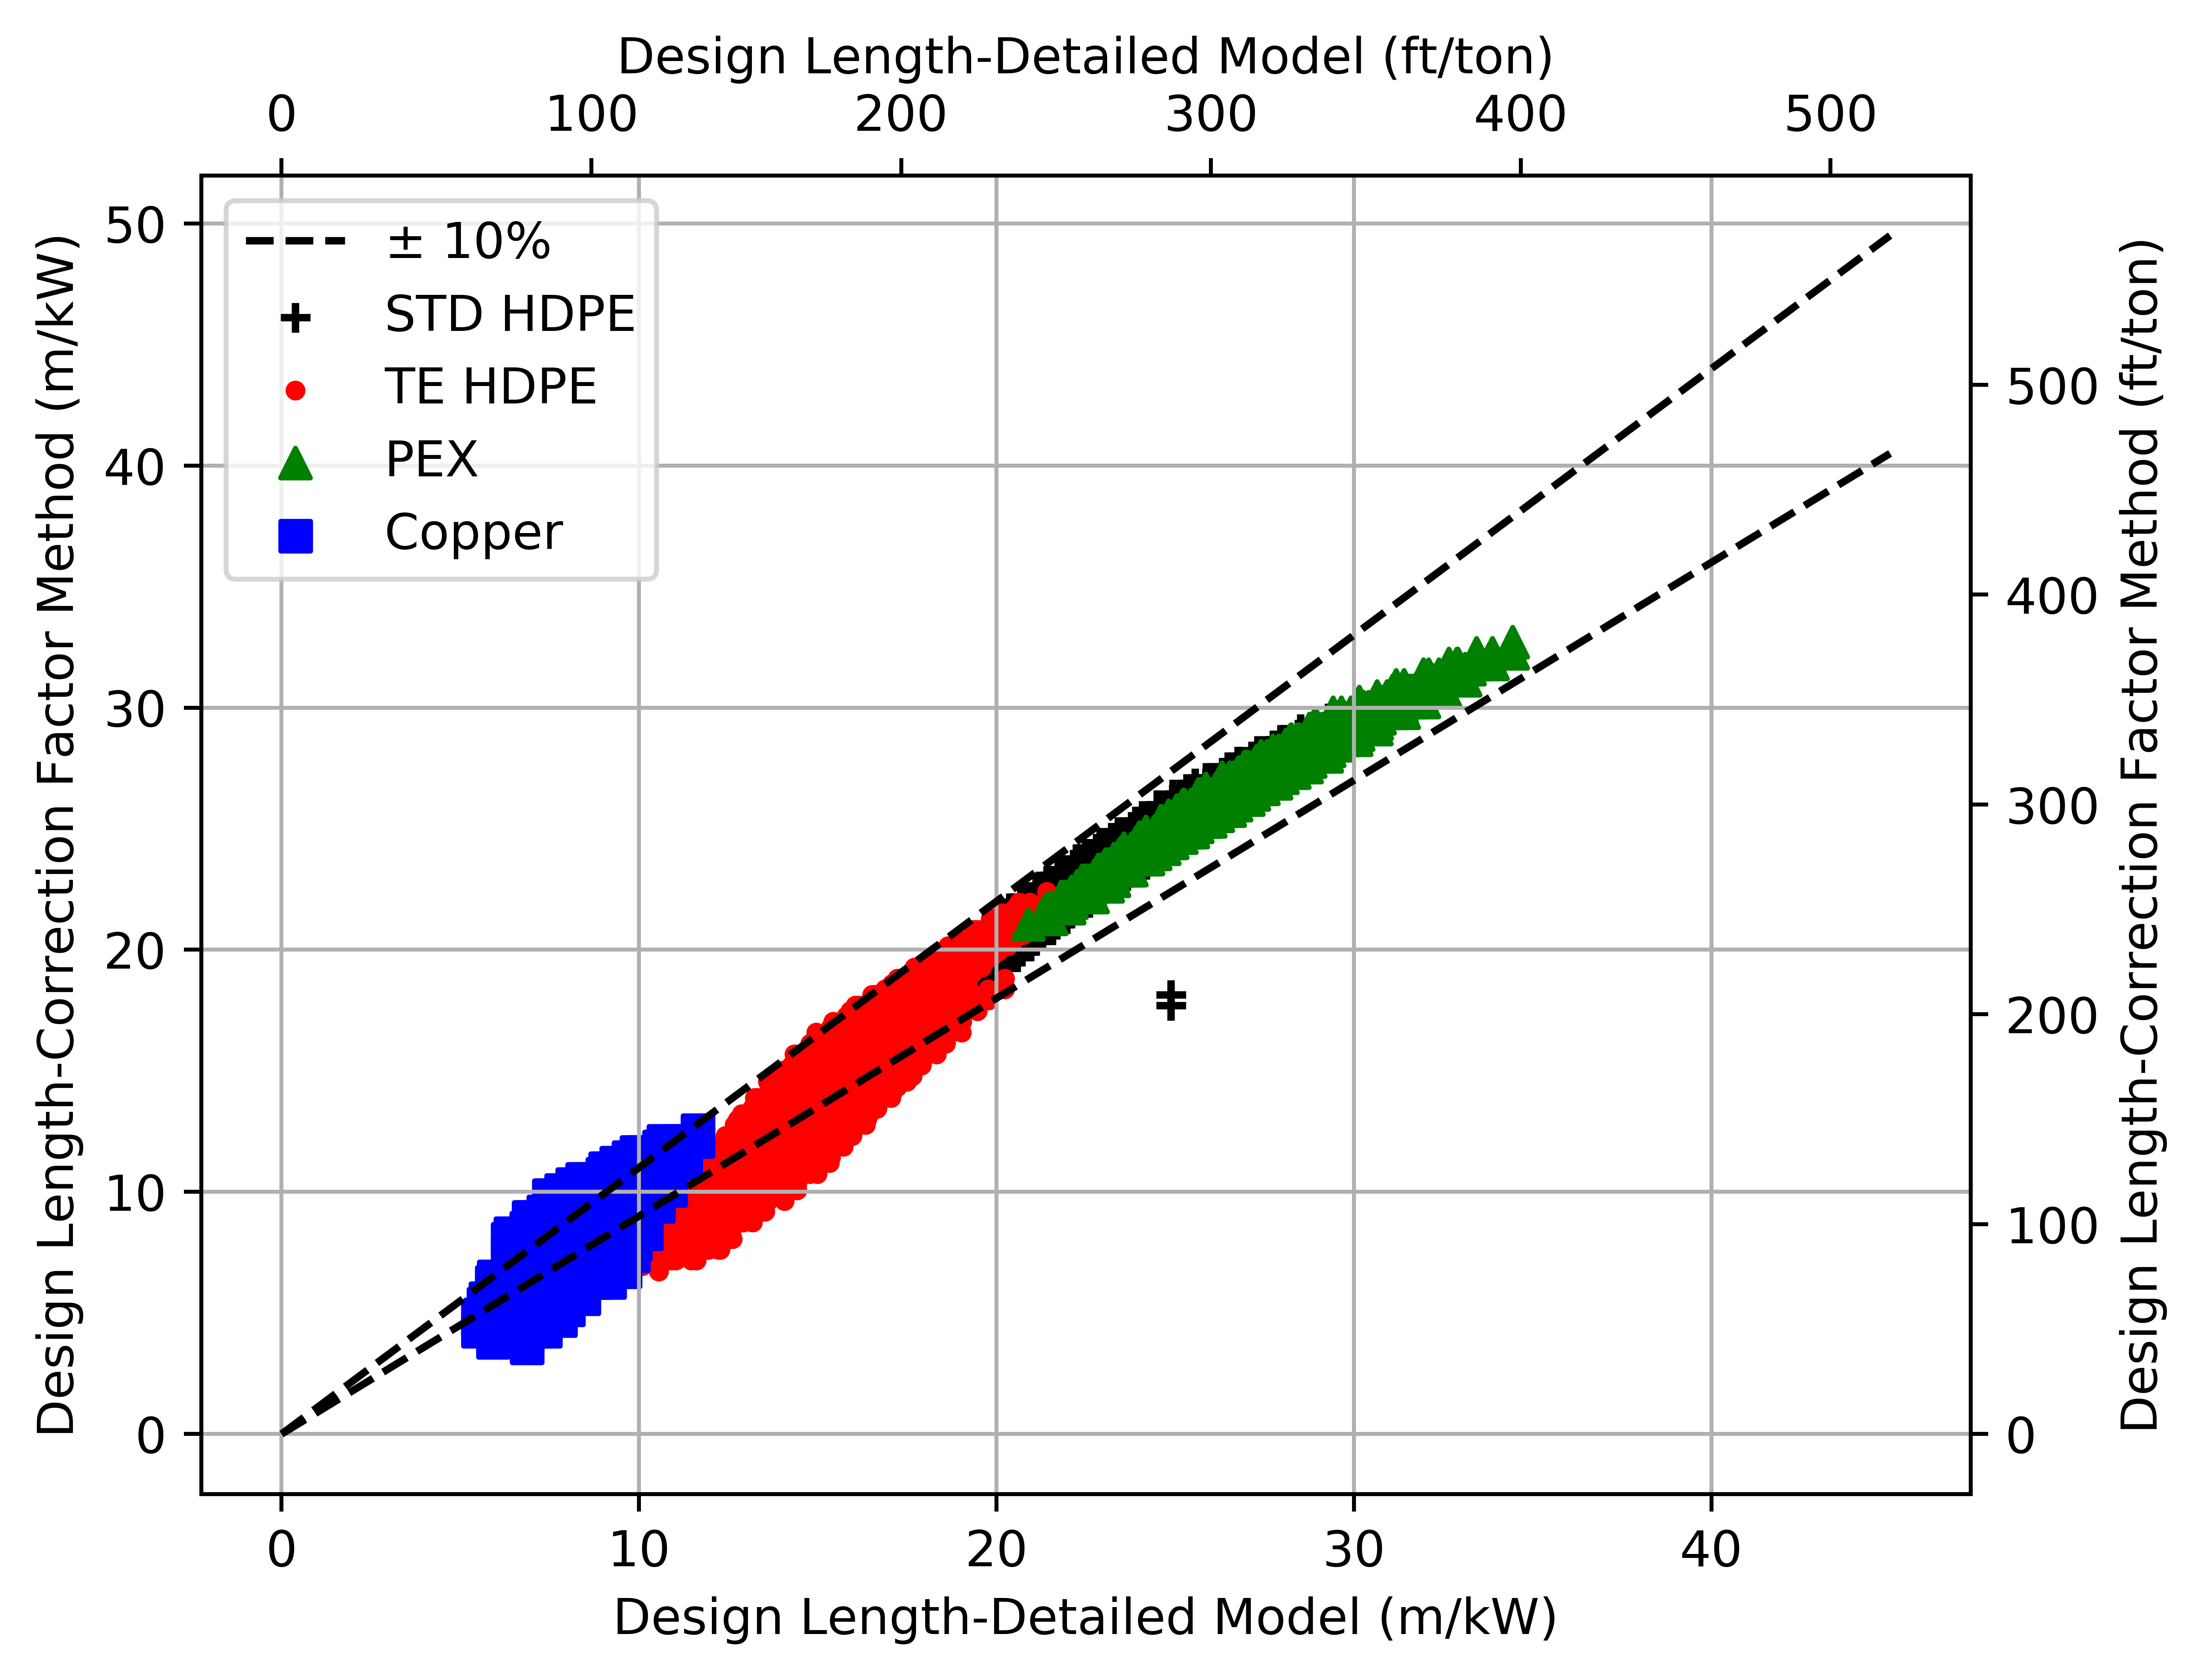
\includegraphics[width=0.75\textwidth]{Comparison.png}
    \caption{Something cool}
    \label{fig:cool figure}
\end{figure}

\section{Literature Review}

\lipsum[1]

\subsection{Literature on Subject A}

\lipsum[1]

\subsection{Literature on Subject B}

\chapter{Methods}
\label{ch:Methods}

\section{Current Methods}

Here's a table which was generated by \LaTeX. Entering this information manually can be tedious, and prone to error. Use a website like \url{http://www.tablesgenerator.com/} to enter data and automatically generate the \LaTeX code for the table.

\begin{table}[h]
\centering
\caption{Some Data}
\label{tab:data}
\begin{tabular}{|l|c|c|c|c|c|}
\hline
                     &              & \textbf{j=1} & \textbf{j=2} & \textbf{j=3} & \textbf{j=4} \\ \hline
\textbf{Floor-South} & \textbf{i=1} & 0.00000      & 0.00000      & 0.19957      & 0.22824      \\ \hline
\textbf{Floor-North} & \textbf{i=2} & 0.00000      & 0.00000      & 0.05763      & 0.20588      \\ \hline
\textbf{South Wall}  & \textbf{i=3} & 0.19049      & 0.00891      & 0.00000      & 0.22078      \\ \hline
\textbf{East Wall}   & \textbf{i=4} & 0.17429      & 0.02546      & 0.17663      & 0.00000      \\ \hline
\end{tabular}
\end{table}

\section{Better Methods}

\lipsum[1]

\begin{figure}
    \centering
    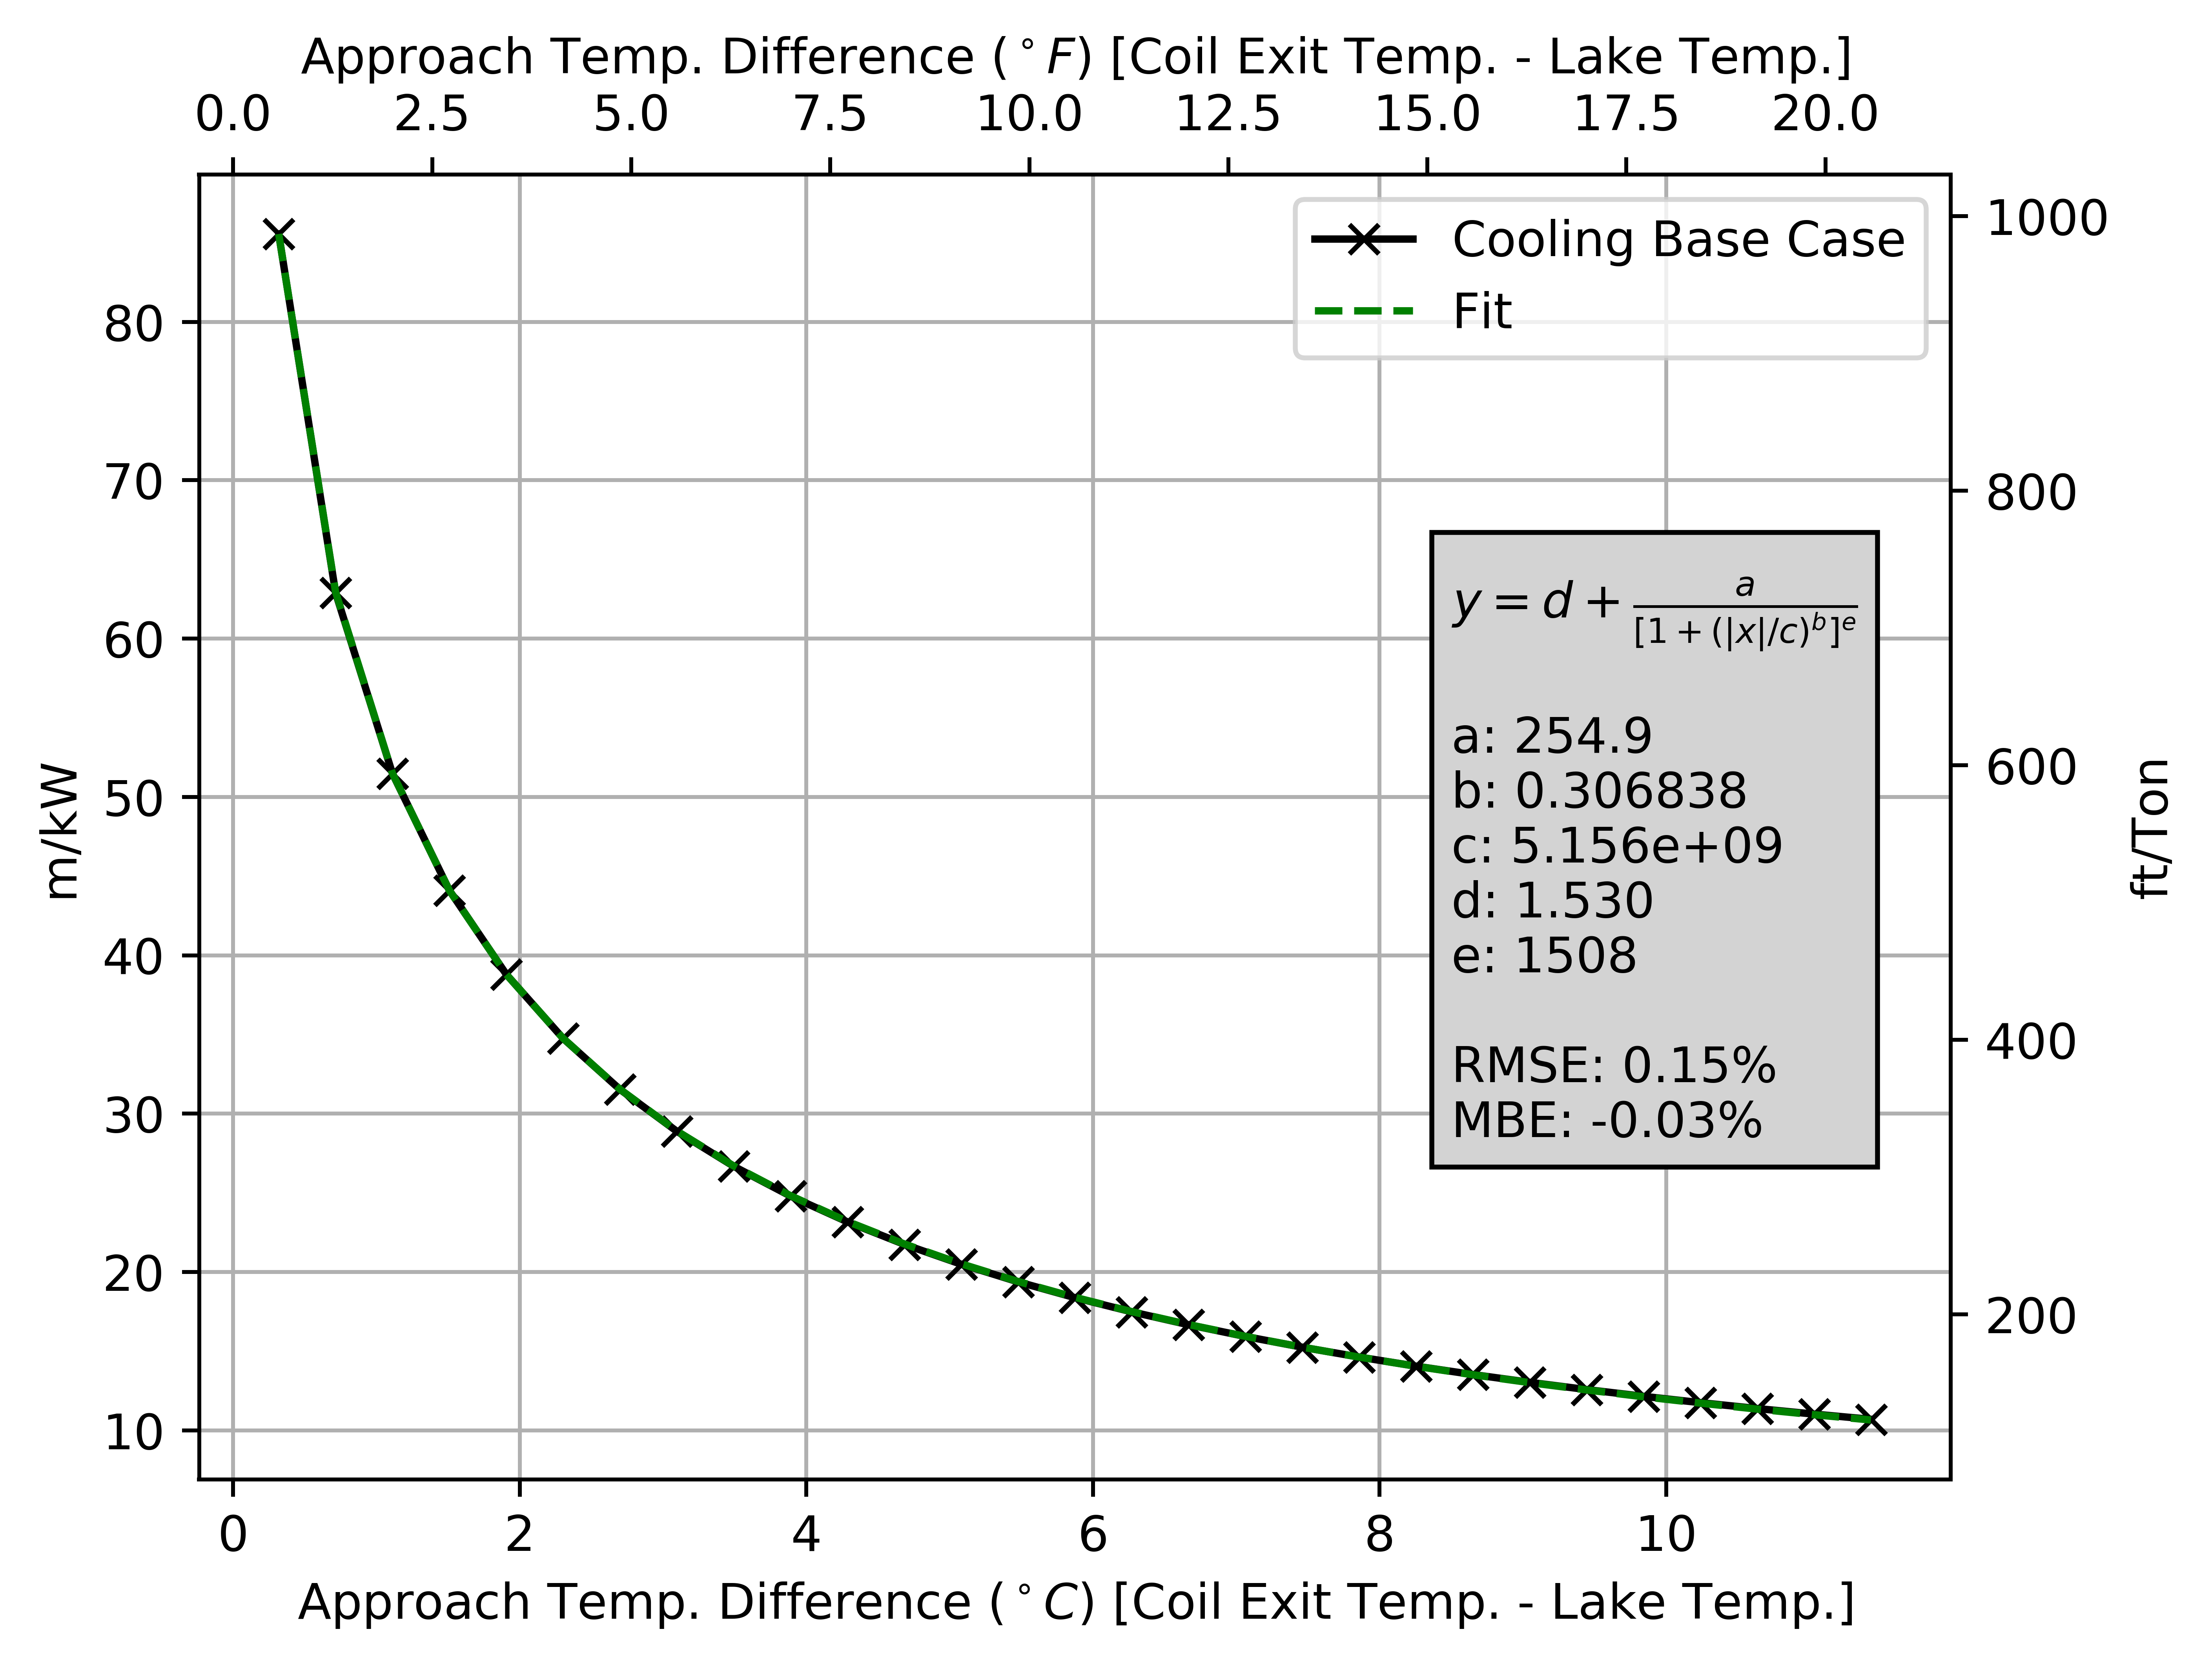
\includegraphics[width=0.75\textwidth]{Cooling_BaseCase_CurveFit.png}
    \caption{Another cool figure}
    \label{fig:another cool figure}
\end{figure}

\chapter{Results}
\label{ch:Results}

\section{My Results}

You can also add tables which have been generated outside of \LaTeX. Below is one example.

\begin{table}[h]
\centering
\caption{Some (more) Data}
\label{tab:more data}
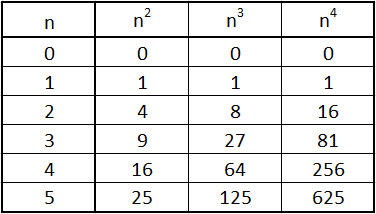
\includegraphics[width=0.75\textwidth]{Table.PNG}
\end{table}

\section{More Results}

Look, here's an equation.

\begin{equation}
    E = m \cdot c^2
\end{equation}

Here are more equations using the \texttt{align} environment.

\begin{align}
    c_p &\approx \frac{Q}{m \cdot dT/dt} \\
    m &= \rho V
\end{align}



%===================== bibliography ============================================
%\nocite{*} %leave this to put ALL references in the bibliography
\newpage
\renewcommand\bibname{\centering References}
\addcontentsline{toc}{chapter}{References}
\bibliography{References/References} %use main dissertation bibtex file
\bibliographystyle{apa}

% uncomment to print all refs in BibTex lib
%\nocite{*}

%====================== appendices ==============================================
\appendix
\singlespace
\chapter{Surface Data}
\label{ch:App:surface data}

\begin{table}[h]
\centering
\caption{Surface data}
\label{tab:surface data}
\begin{tabular}{|l|c|}
\hline
                        & \begin{tabular}[c]{@{}c@{}}Surface Fluxes\\  W/m2\end{tabular} \\ \hline
Floor-South             & -172.0                                                         \\ \hline
Floor-North             & -158.1                                                         \\ \hline
South Wall              & -25.7                                                          \\ \hline
East Wall               & -29.3                                                          \\ \hline
West Wall-South         & -33.1                                                          \\ \hline
West Wall-North         & -130.6                                                         \\ \hline
North Wall-Bottom       & -58.0                                                          \\ \hline
North Wall-Below Window & -166.7                                                         \\ \hline
Window                  & -201.7                                                         \\ \hline
North Wall-Above Window & 52.3                                                           \\ \hline
Ceiling                 & 227.6                                                          \\ \hline
Sauna-South Face        & 166.4                                                          \\ \hline
Sauna-East Face         & 187.7                                                          \\ \hline
Hot Rocks               & 5343.1                                                         \\ \hline
\end{tabular}
\end{table}

\chapter{Other important information}
\lipsum[3]

\begin{figure}[htbp!]
    \centering
    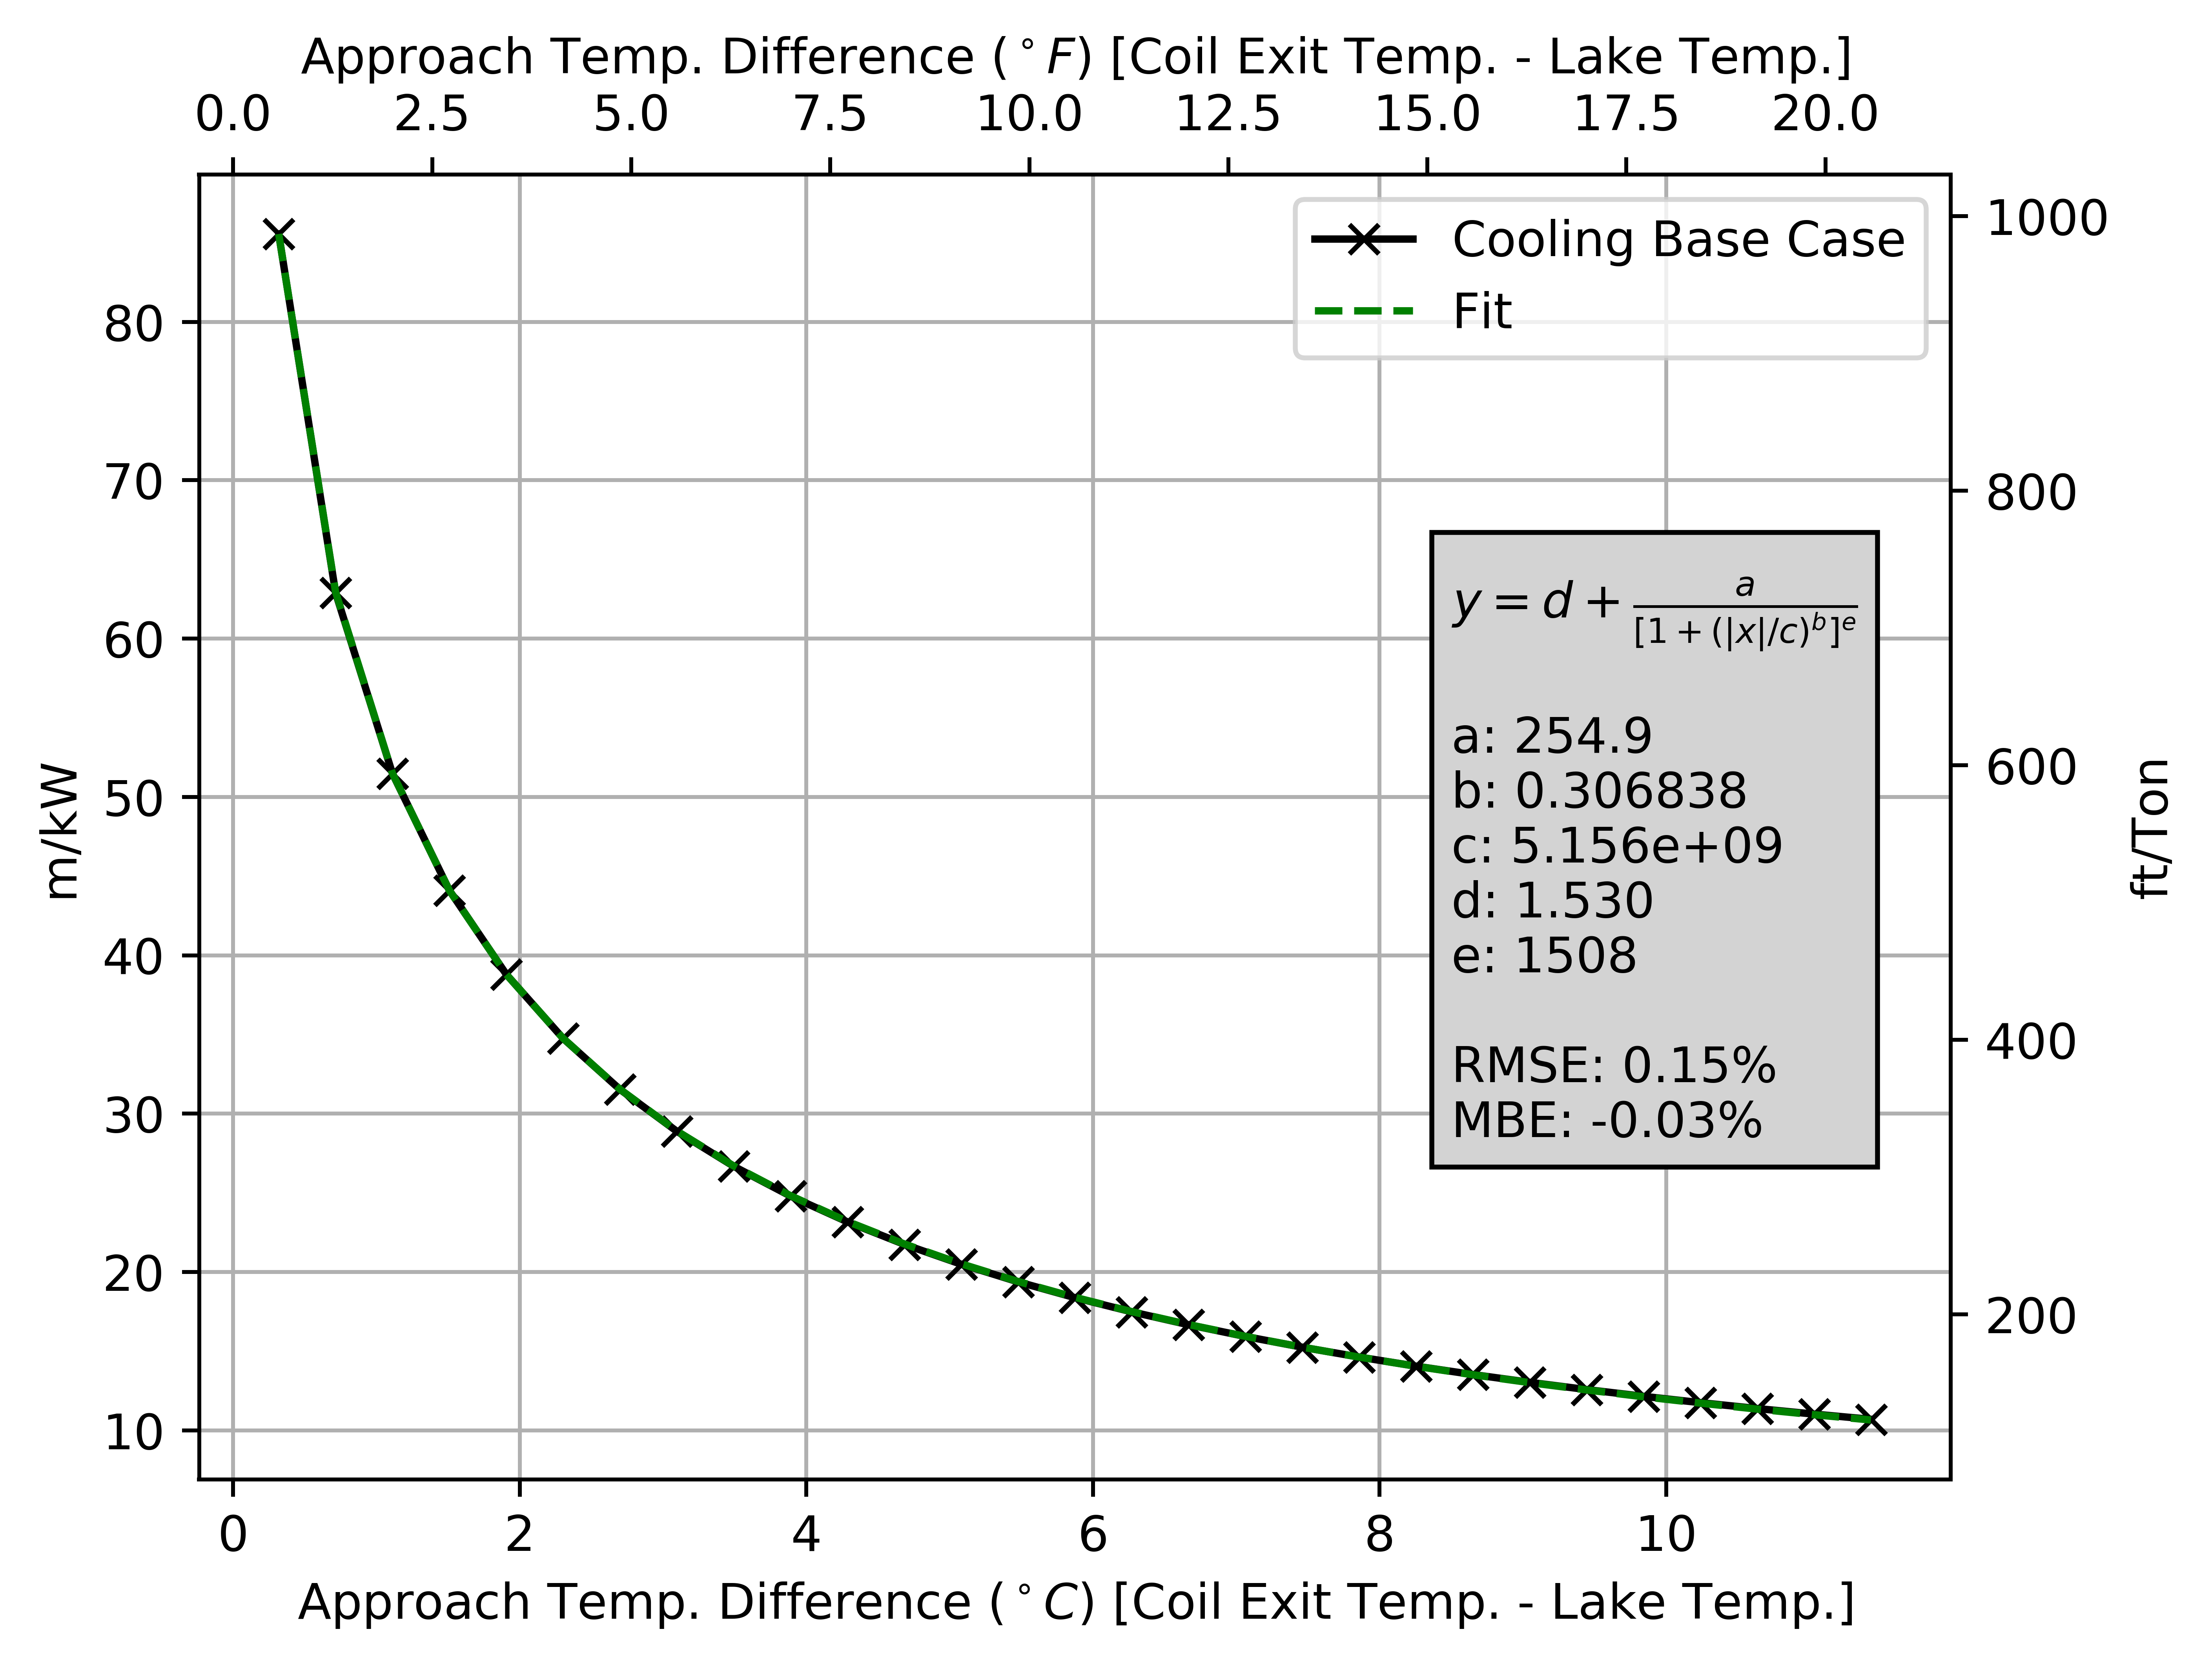
\includegraphics[width=0.75\textwidth]{Cooling_BaseCase_CurveFit.png}
    \caption{Another cool figure (in the appendix)}
    \label{fig:another cool figure in appendix}
\end{figure}


%====================== vita ====================================================
\newpage
\begin{vita}{JOHN Q. DOE}{Doctor of Philosophy}{Rocket Science} %Creates vita
    \vitaitem{Personal Data:} Born in Stillwater, Oklahoma in February 2000.
    \vitaitem{Education:} \\ Received a Bachelors of Science in Aeronautics at Oklahoma State University in July 2010. \\
Completed the requirements for the degree of Doctor of Philosophy with a major in Rocket Science at Oklahoma State University in July 2010.
    \vitaitem{Experience:} \\ Works on a ranch, and loves long walks on the beach.

    \vitaitem{Professional Affiliations:} \\ Fellow AIAA
\end{vita}


\end{document}
